%% ------------------------------------------------------- %%
%% Rodin SMT plugin example
%% ------------------------------------------------------- %%
\section{Rodin SMT plugin example}
The RODIN plugin introduced in this document is still a prototype. For the moment, it can handle some basic arithmetic proof obligations but still needs to be improved to be much more efficient.
 
Here is an overview of how the plugin works:

\paragraph{Rodin preferences}
To use the plugin, the user must set up SMT preferences by reaching the Windows/Preferences Menu of Rodin (Figure \ref{RodinSMTPreferences}).

\paragraph{Solver preference}
The user must provide info on solvers just like if a preprocessing is used or not. Pushing the \textit{Add} button leads to the following window (Figure \ref{NewSolverSMTPreferences}):

\paragraph{Solver preference creation}
The user must provide following info :

\begin{itemize}
\item An Id,
\item A path,
\item Arguments used to call the solver,
\item On which SMT-LIB version the solver will be used.   
\end{itemize}

\paragraph{Solver selection}
The user must then select the solver that will be used ( \textit{Select} button in Figure \ref{RodinSMTPreferences}):

\paragraph{Solver launching}
To launch the SMT solver on the selected Proof Obligation, the user must press the SMT button (Figure \ref{LaunchSMT}):


\paragraph{Solver result}
If the SMT solver suceeds, the status will be updated in the proof tree (Figure \ref{SMTResults}):

\begin{figure}[!p]
\centering
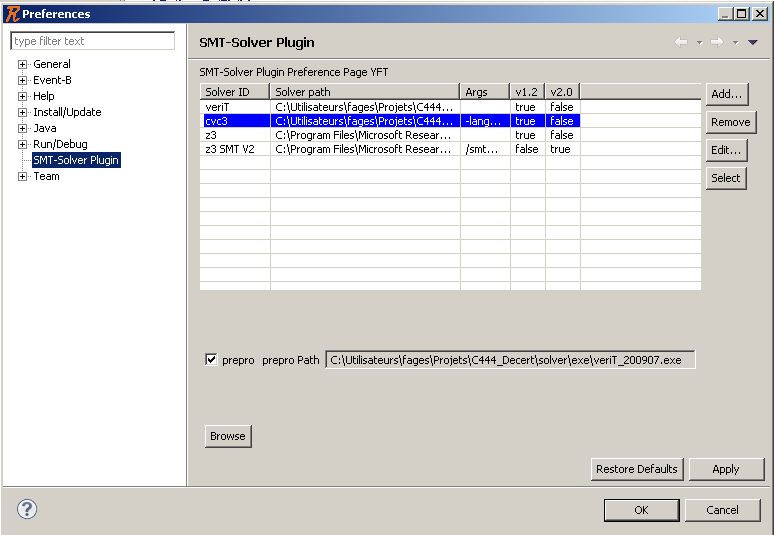
\includegraphics[scale=0.5]{preferences2.PNG}
\caption{Rodin SMT preferences page} 
\label{RodinSMTPreferences}
\end{figure}

\begin{figure}[!p]
\centering
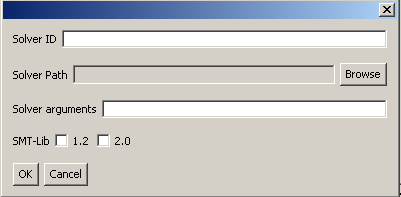
\includegraphics[scale=0.5]{preferences3.PNG}
\caption{Rodin SMT preferences page, new solver} 
\label{NewSolverSMTPreferences}
\end{figure}

\begin{figure}[!p]
\centering
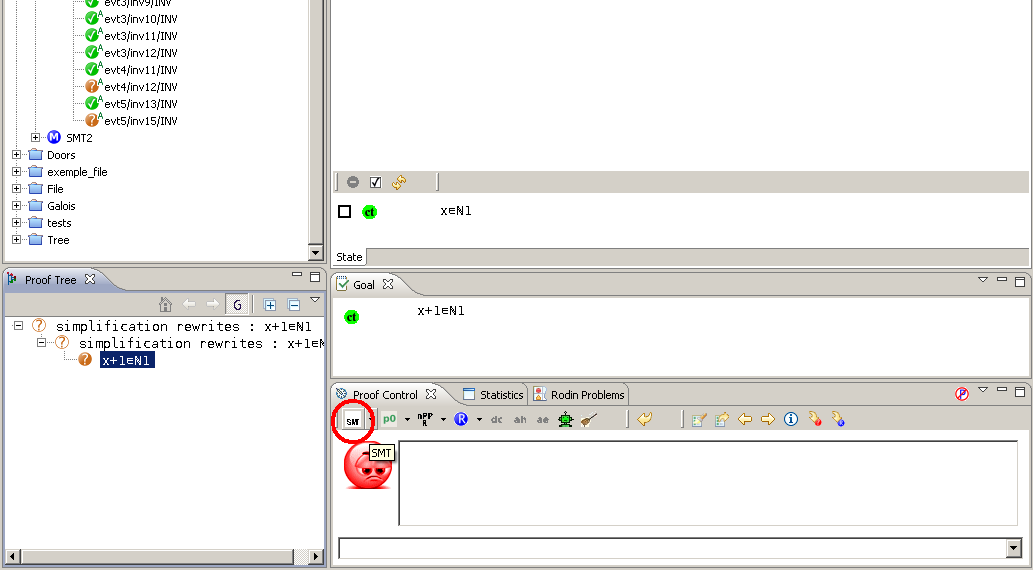
\includegraphics[scale=0.5]{smt.PNG}
\caption{Rodin SMT button} 
\label{LaunchSMT}
\end{figure}

\begin{figure}[!p]
\centering
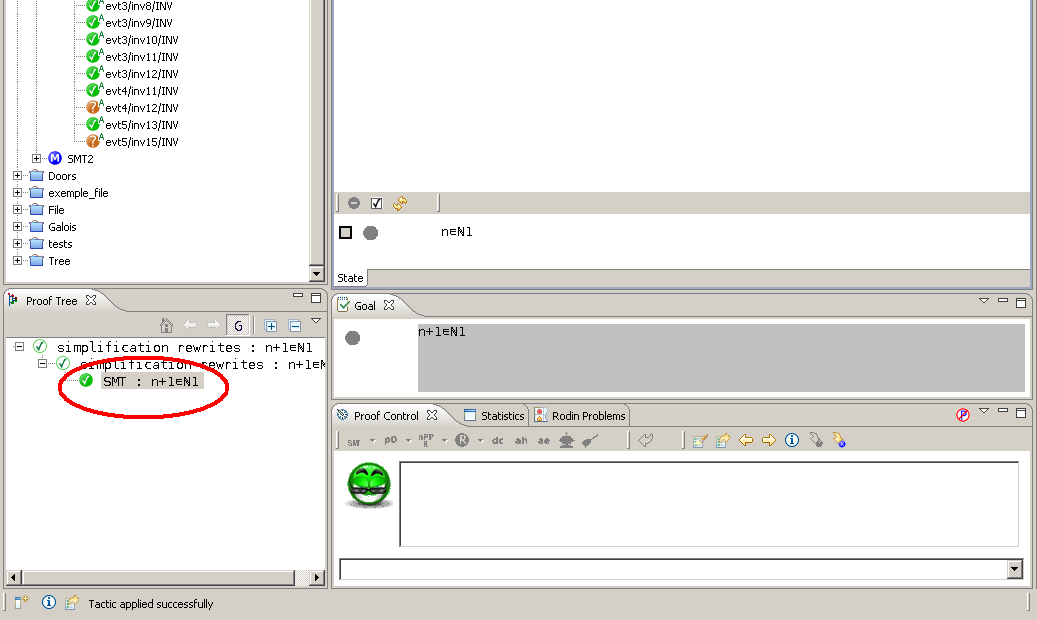
\includegraphics[scale=0.5]{smt2.PNG}
\caption{Rodin SMT results} 
\label{SMTResults}
\end{figure}


